%
% Copyright 2018 Joel Feldman, Andrew Rechnitzer and Elyse Yeager.
% This work is licensed under a Creative Commons Attribution-NonCommercial-ShareAlike 4.0 International License.
% https://creativecommons.org/licenses/by-nc-sa/4.0/
%
\questionheader{ex:s3.4}
%%%%%%%%%%%%%%%%%%
\subsection*{More Problems for Section 3.4}
%%%%%%%%%%%%%%%%%%
%%%%%%%%%%%%%%%%%%
\subsection*{\Conceptual}
%%%%%%%%%%%%%%%%%%


\begin{question}[2015Q]
Consider a function $f(x)$ whose third order Maclaurin polynomial is $4 +
3x^2 + \frac{1}{2}x^3$.
 What is $f'(0)$? What is $f''(0)$?
\end{question}
\begin{hint} Compare the given polynomial to the definition of a Maclaurin polynomial.
\end{hint}
\begin{answer} $f'(0)=0$ and $f''(0)=6$.
\end{answer}
\begin{solution}
The third Maclaurin polynomial for $f(x)$ is
\begin{align*}
f(0) + f'(0)x +\frac{f''(0)}{2}\cdot x^2 + \frac{f'''(0)}{6}\cdot x^3
&=4+3x^2+\frac{1}{2}x^3.
\end{align*}
The coefficient of $x$ is $f'(0)$ on  one side, and $0$ on the other, so
 $f'(0)=0$.\\
 The coefficient of $x^2$ is $\dfrac{1}{2}f''(0)$ on  one side, and $3$ on the other, so
 $f''(0)=6$.
\end{solution}


\begin{question}[2015Q]
Consider a function $h(x)$ whose third order Maclaurin polynomial is
$1+4x-\dfrac{1}{3}x^2 + \dfrac{2}{3}x^3$. What is $h^{(3)}(0)$?
\end{question}
\begin{answer}
$4$
\end{answer}
\begin{solution}
The third Maclaurin polynomial for $h(x)$ is
\begin{align*}
    h(0) + h'(0)x +\frac{h''(0)}{2}\cdot x^2 + \frac{h^{(3)}(0)}{3!}\cdot x^3
    &= 1+4x-\frac{1}{3}x^2 + \frac{2}{3}x^3
\end{align*}
 The coefficient of $x^3$ is $\dfrac{1}{3!}h^{(3)}(0)$ on  one side, and $\dfrac{2}{3}$ on the other. \\ Thus $ \dfrac{h^{(3)}(0)}{6}=\dfrac{2}{3}$, so $h^{(3)}(0)=6\cdot\dfrac{2}{3} = 4$.
\end{solution}




\begin{question}[2015Q]
The third order Taylor polynomial of $h(x)$ about $x=2$ is $3 + \dfrac{1}{2}(x-2) + 2(x-2)^3$.

What is $h'(2)$?
What is $h''(2)$?
\end{question}
\begin{hint}
Compare the given polynomial to the definition of a Taylor polynomial.
\end{hint}
\begin{answer}
$h'(2)=\dfrac{1}{2}$,
$h''(2)=0$
\end{answer}
\begin{solution}
The third order Taylor polynomial for $h(x)$ about $x=2$ is
\[
h(2) + h'(2)(x-2) +\frac{h''(2)}{2}\cdot (x-2)^2 + \frac{h'''(2)}{6}\cdot (x-2)^3\]
 The coefficient of $(x-2)$ is $h'(2)$ in the definition, and
  $\dfrac{1}{2}$ in the given function, so $h'(2)=\dfrac{1}{2}$.

  The coefficient of $(x-2)^2$ is $~\dfrac{1}{2}h''(2)~$ in the definition, and
  $0$ in the given function, so $h'(2)=0$.
\end{solution}



%%%%%%%%%%%%%%%%%%
\subsection*{\Procedural}
%%%%%%%%%%%%%%%%%%

\begin{Mquestion}[1997D]
The function $f(x)$ has the property that $f(3)=2,\ f'(3)=4$
and $f''(3)=-10$.
\begin{enumerate}[(a)]
\item Use the linear approximation to $f(x)$ centred at $x=3$ to
approximate $f(2.98)$.
\item  Use the quadratic approximation to $f(x)$ centred at $x=3$ to
approximate $f(2.98)$.\end{enumerate}
\end{Mquestion}
\begin{answer}
(a) $1.92$\qquad
(b) $1.918$
\end{answer}
\begin{solution}
\begin{enumerate}[(a)]
\item For $x$ near 3,
\[
f(x)\approx f(3)+f'(3)(x-3)=2+4(x-3)
\]
In particular
\[
f(2.98)\approx 2+4(2.98-3)=2-0.08=1.92
\]

\item
For $x$ near 3,
\begin{align*}
f(x)&\approx f(3)+f'(3)(x-3)+\frac{1}{2} f''(3)(x-3)^2\\
&=2+4(x-3)-\frac{1}{2} 10(x-3)^2
\intertext{In particular}
f(2.98)&\approx 2+4(2.98-3)-5(2.98-3)^2\\
&=2-0.08-0.002={1.918}
\end{align*}
\end{enumerate}
\end{solution}

\begin{Mquestion}[2010H]
Use the tangent line to the graph of $y = x^{1/3}$ at
$x = 8$ to find an approximate value for $10^{1/3}$. Is the
approximation too large or too small?
\end{Mquestion}
\begin{hint}
You can use the error formula to determine whether the approximation is too large or too small.
\end{hint}
\begin{answer}
$10^{1/3}\approx\dfrac{13}{6}$; this approximation is too big.
\end{answer}
\begin{solution}
 Let's name $g(x)=x^{1/3}$. Then $g'(x)=\dfrac{1}{3} x^{-2/3}$
and $g''(x)=-\dfrac{2}{9} x^{-5/3}$.\\
 In particular, $g(8)=2$,
$g'(8)=\dfrac{1}{12}$, and $g''(x)<0$ for all $x>0$.

The tangent line
approximation to $10^{1/3}$ is
\begin{align*}
g(10)&\approx g(8)+g'(8)(10-8)\\
&=2+\dfrac{1}{12}(2)=\dfrac{13}{6}
\intertext{Using the error formula:}
g(10)&=g(8)+g'(8)(10-8)+\half g''(c)(10-8)^2
\end{align*}
for some $8<c<10$. Since $g''(c)=-\dfrac{2}{9c^{5/3}}$,  $g''(c)$ is negative, so
$g(10)$ is $\dfrac{13}{6} $ plus some \emph{negative} quantity. So,
the tangent line approximation is too
big.
\end{solution}



\begin{question}[2015Q]
 Estimate $\sqrt{2}$ using a linear approximation.
\end{question}
\begin{hint} Use the function $f(x)=\sqrt{x}$.
\end{hint}
\begin{answer} $\sqrt{2}\approx \dfrac{3}{2}$
\end{answer}
\begin{solution}
We use the function $f(x)=\sqrt{x}$ and point $a=1$ as the centre of our
approximation, since we can easily calculate
\begin{align*}
  f(a)&=f(1)=\sqrt{1}=1.
\end{align*}
We compute $f'(x)=\dfrac{1}{2\sqrt{x}}$, so
\begin{align*}
f'(1)&=\frac{1}{2\sqrt{1}}=\frac{1}{2}.
\end{align*}
So, a linear approximation of $\sqrt{2}=f(2)$ is
\begin{align*}
\sqrt{2}&\approx T_1(2)= f(1) + f'(1)\cdot (2-1)\\
&=1+\frac{1}{2}=\frac{3}{2}.
\end{align*}
\end{solution}



\begin{question}[2015Q]
Estimate $\sqrt[3]{26}$ using a linear approximation.
\end{question}
\begin{hint} Use the function $f(x)=x^{1/3}$. What is a good choice of centre?
\end{hint}
\begin{answer}
  $ \sqrt[3]{26}\approx \dfrac{80}{27}$
\end{answer}
\begin{solution}
We use the function $f(x)=x^{1/3}$ and point $a=27$ as the centre of our
approximation since we can easily compute
\begin{align*}
    f(27)&=3
\end{align*}
We compute $f'(x)=\dfrac{1}{3} x^{-2/3}$, so
\begin{align*}
    f'(27)&= \frac{1}{3} \cdot (27)^{-2/3} = \frac{1}{27}
\end{align*}
So, the linear approximation of $26^{1/3} = f(26)$ is
\begin{align*}
    26^{1/3}&\approx T_1\left(26\right) = f(27) + f'(27)\cdot (26-27) \\
  &= 3 - \frac{1}{27} = \frac{80}{27}
\end{align*}
\end{solution}




\begin{question}[2015Q]
Estimate $(10.1)^5$ using a linear approximation.
\end{question}
\begin{hint} Try using the function $f(x)=x^5$.
\end{hint}
\begin{answer}
$(10.1)^5 \approx 105,000$
\end{answer}
\begin{solution}
We use the function $f(x)=x^5$ and point $a=10$ as the centre of our
approximation since we know that $f(a)=f(10)=10^5$.

Since $f'(x) = 5x^4$ we have $f'(10) = 50,000$.

So, a linear approximation of $10.1^5$ is
\begin{align*}
T_1(10.1)&= f(10) + f'(10)\cdot (10.1-10) \\
 &= 100,000 + 50,000 \cdot 0.1 = 105,000\,.
\end{align*}
\end{solution}




\begin{question}[2015Q]
Estimate $\sin\left(\dfrac{101\pi}{100}\right)$ using a linear approximation. (Leave
your answer in terms of $\pi$.)
\end{question}
\begin{hint} If you use the function $f(x)=\sin(x)$, what is a good centre?
\end{hint}
\begin{answer}
$\sin\left(\dfrac{101\pi}{100}\right) \approx -\dfrac{\pi}{100}$
\end{answer}
\begin{solution}
We use the function $f(x)=\sin(x)$ and point $a=\pi$ as the centre of our
approximation since we know that
\begin{align*}
    \sin(a)&=f(\pi)=\sin{\pi}=0.
\end{align*}
and $\pi$ is reasonably close to $\dfrac{101\pi}{100}$.\\
We compute $f'(x)=\cos(x)$, so
\begin{align*}
    f'(\pi)&=\cos(\pi) = -1.
\intertext{So, the linear approximation of
    $\sin\left(\frac{101\pi}{100}\right) $ is}
    f\left(\frac{101\pi}{100}\right)&\approx
    T_1\left(\frac{101\pi}{100}\right)\\
  &= f(\pi) + f'(\pi)\cdot \left(\frac{101\pi}{100}-\pi\right) \\
  &=0+(-1)\cdot\frac{\pi}{100}=-\frac{\pi}{100}.
\end{align*}
\end{solution}


\begin{Mquestion}[2009H]
 Use a linear approximation to estimate $\arctan(1.1)$, using
$\arctan 1 = \dfrac{\pi}{4}$.
\end{Mquestion}
\begin{hint}
Recall $\ds\diff{}{x}\left\{\arctan x\right\} = \dfrac{1}{1+x^2}$.
\end{hint}
\begin{answer}
$\arctan(1.1)\approx\left(\dfrac{\pi}{4}+\dfrac{1}{20}\right)$
\end{answer}
\begin{solution}
Set $f(x)=\arctan(x)$. Then $f'(x)=\dfrac{1}{1+x^2}$, so
$f'(1)=\dfrac{1}{2}$ and
$$
f(1.1)\approx f(1)+f'(1)(1.1-1)=\frac{\pi}{4}+\frac{1}{20}
$$
\end{solution}


\begin{question}[2007H]
 Use a linear approximation to estimate $(2.001)^3$.
Write your answer in the form $n/1000$ where $n$ is an integer.
\end{question}
\begin{hint}
Try using the function $f(x)=(2+x)^3$.
\end{hint}
\begin{answer} $\dfrac{8012}{1000}$
\end{answer}
\begin{solution}
Set $f(x)=(2+x)^3$, so we are approximating $f(0.001)$. \\
The obvious choice of $a$ is $a=0$.

 Then $f'(x)=3(2+x)^2$, so
$$
(2.001)^3=f(0.001)\approx f(0)+f'(0)(0.001-0)
=8+\frac{12}{1000}=\frac{8012}{1000}
$$

Remark: if we had chosen $f(x)=x^3$ and $a=2$, the result would have been exactly the same.
\end{solution}


\begin{question}[2006H]
Using a suitable linear approximation, estimate
$(8.06)^{2/3}$. Give your answer as a fraction in which both the
numerator and denominator are integers.
\end{question}
\begin{hint}
You can try using $f(x)=(8+x)^{1/3}$. What is a suitable centre for your approximation?
\end{hint}
\begin{answer}
$(8.06)^{2/3}\approx\dfrac{402}{100}=\dfrac{201}{50}$
\end{answer}
\begin{solution}
We set $f(x)=(8+x)^{2/3}$, and choose $a=0$ as our centre.\\
Then $f'(x)=\dfrac{2}{3}(8+x)^{-1/3}$, so that
\begin{align*}
(8.06)^{2/3}=f(0.06)&\approx f(0)+f'(0)\cdot 0.06\\
&=8^{2/3}+\frac{2}{3}8^{-1/3}\cdot 0.06\\
&=\sqrt[3]{8}^2+\frac{2}{3\sqrt[3]{8}}\cdot 0.06\\
&=2^2+\frac{2}{3\cdot 2}\cdot 0.06\\
&=4+\frac{1}{3}\cdot 0.06\\&=4.02=\frac{402}{100}\end{align*}
\end{solution}


\begin{question}[2006H]
Find the third--order Taylor polynomial for
$f(x)=(1 - 3x)^{-1/3}$ around $x = 0$.
\end{question}
\begin{hint}
This is the same as the Maclaurin polynomial.
\end{hint}
\begin{answer}
$1 + x +2x^2+\dfrac{14}{3}x^3$
\end{answer}
\begin{solution}
We begin by finding the derivatives of $f$ at $x=0$.
\begin{align*} f(x)&=(1 - 3x)^{-1/3} & f(0) & = 1 \\
 f'(x)&=(-3)\frac{-1}{3}(1 - 3x)^{-4/3}=(1-3x)^{-4/3} & f'(0) & = 1 \\
 f''(x)&=(-3)\frac{-4}{3}(1-3x)^{-7/3}={4}(1 - 3x)^{-7/3} & f''(0) & = 4 \\
 f^{(3)}(x)&=(-3)(4)\frac{-7}{3}(1-3x)^{-10/3}=28(1 - 3x)^{-10/3} & f^{(3)}(0) & = 28 \\
\end{align*}
Plugging these into the definition of a Taylor Polynomial, we find that the third--order Taylor polynomial for $f$ around $x = 0$ is
\begin{align*}
T_3(x)&=1+x+\frac{4}{2!}x^2+\frac{28}{3!}x^3\\
&=1 + x +2x^2+\frac{14}{3}x^3
\end{align*}
\end{solution}



\begin{question}[2015Q]
Consider a function $f(x)$ which has $f^{(3)}(x)=\dfrac{x}{22-x^2}$.  Show
that when we approximate $f(2)$ using its second order Taylor polynomial at $a=1$, the
absolute value of the error is less than $\frac{1}{50}=0.02$.
\end{question}
\begin{hint}
This is a straightforward application of Equation~\ref*{eq:taylorErrorN}.
\end{hint}
\begin{answer}
\begin{itemize}
 \item By  Equation~\ref*{eq:taylorErrorN}, the absolute value of the error is
\[\left|\frac{f'''(c)}{3!}\cdot (2-1)^3\right|
= \left|\frac{c}{6(22-c^2)}\right|\]
for some $c \in (1,2)$.
\item When $1\leq c\leq2$, we know that $18 \leq 22-c^2 \leq 21$, and that numerator and denominator are non-negative, so
\begin{align*}
\left|\frac{c}{6(22-c^2)}\right|
  &=\frac{c}{6(22-c^2)}
  \leq \frac{2}{6(22-c^2)}  \leq \frac{2}{6\cdot 18} \\
  & = \frac{1}{54} \leq \frac{1}{50}
\end{align*}
as required.

\item Alternatively, notice that $c$ is an increasing function of
$c$, while $22-c^2$ is a decreasing function of $c$. Hence the fraction is an
increasing function of $c$ and takes its largest value at $c=2$. Hence
\begin{align*}
\left|\frac{c}{6(22-c^2)}\right|
& \leq \frac{2}{6\times 18} = \frac{1}{54} \leq \frac{1}{50}.
\end{align*}
\end{itemize}
\end{answer}
\begin{solution}
\begin{itemize}
 \item By  Equation~\ref*{eq:taylorErrorN}, the absolute value of the error is
\[\left|\frac{f'''(c)}{3!}\cdot (2-1)^3\right|
= \left|\frac{c}{6(22-c^2)}\right|\]
for some $c \in (1,2)$.
\item When $1\leq c\leq2$, we know that $18 \leq 22-c^2 \leq 21$, and that numerator and denominator are non-negative, so
\begin{align*}
\left|\frac{c}{6(22-c^2)}\right|
  &=\frac{c}{6(22-c^2)}
  \leq \frac{2}{6(22-c^2)}  \leq \frac{2}{6\cdot 18} \\
  & = \frac{1}{54} \leq \frac{1}{50}
\end{align*}
as required.

\item Alternatively, notice that $c$ is an increasing function of
$c$, while $22-c^2$ is a decreasing function of $c$. Hence the fraction is an
increasing function of $c$ and takes its largest value at $c=2$. Hence
\begin{align*}
\left|\frac{c}{6(22-c^2)}\right|
& \leq \frac{2}{6\times 18} = \frac{1}{54} \leq \frac{1}{50}.
\end{align*}
\end{itemize}
\end{solution}





\begin{Mquestion}[2015Q]
Consider a function $f(x)$ which has $f^{(4)}(x)=\dfrac{\cos(x^2)}{3-x}$.  Show
that when we approximate $f(0.5)$ using its third order Maclaurin polynomial,
the absolute value of the error is less than $\frac{1}{500}=0.002$.
\end{Mquestion}
\begin{answer}
\begin{itemize}
 \item By Equation~\ref*{eq:taylorErrorN}, there is $c\in(0,0.5)$ such
that the error is
\begin{align*}
  R_4 &= \frac{f^{(4)}(c)}{4!} (0.5-0)^4 \\
      &= \frac{1}{24\cdot 16} \cdot \frac{\cos(c^2)}{3-c}
\end{align*}

\item For any $c$ we have $|\cos(c^2)| \leq 1$, and for $c<0.5$ we have
$3-c>2.5$,
so that $$\left|\frac{\cos(c^2)}{3-c}\right| \leq \frac{1}{2.5}\,.$$

\item We conclude that
$$ \left| R_4 \right| \leq \frac{1}{2.5\cdot 24\cdot 16} = \frac{1}{60\cdot 16}<\frac{1}{60\cdot 10}=\frac{1}{600}<\frac{1}{500}$$
\end{itemize}
\end{answer}
\begin{solution}
\begin{itemize}
 \item By Equation~\ref*{eq:taylorErrorN}, there is $c\in(0,0.5)$ such
that the error is
\begin{align*}
  R_4 &= \frac{f^{(4)}(c)}{4!} (0.5-0)^4 \\
      &= \frac{1}{24\cdot 16} \cdot \frac{\cos(c^2)}{3-c}
\end{align*}

\item For any $c$ we have $|\cos(c^2)| \leq 1$, and for $c<0.5$ we have
$3-c>2.5$,
so that $$\left|\frac{\cos(c^2)}{3-c}\right| \leq \frac{1}{2.5}\,.$$

\item We conclude that
$$ \left| R_4 \right| \leq \frac{1}{2.5\cdot 24\cdot 16} = \frac{1}{60\cdot 16}<\frac{1}{60\cdot 10}=\frac{1}{600}<\frac{1}{500}$$
\end{itemize}
\end{solution}



\begin{Mquestion}[2015Q]
Consider a function $f(x)$ which has $f^{(3)}(x)=\dfrac{e^{-x}}{8+x^2}$.  Show
that when we approximate $f(1)$ using its second order Maclaurin polynomial, the
absolute value of the error is less than $1/40$.
\end{Mquestion}
\begin{answer}
\begin{itemize}
\item By Equation~\ref*{eq:taylorErrorN}, there is $c\in(0,1)$ such
that the error is
\begin{align*}
\left|\frac{f'''(c)}{3!}\cdot (1-0)^3\right|
&=  \left|\frac{e^{-c}}{6(8+c^2)}\right|.
\end{align*}

\item When $0< c<1$, we know that $1> e^{-c} > e^{-1}$ and
$8 \leq 8+c^2 < 9$, so
\begin{align*}
\left|\frac{e^{-c}}{6(8+c^2)}\right|
  &=\frac{e^{-c}}{6(8+c^2)} \\
  & < \frac{1}{6 |8+c^2|} \\
  & < \frac{1}{6\times 8} = \frac{1}{48} < \frac{1}{40}
\end{align*}
as required.
\end{itemize}
\end{answer}
\begin{solution}
\begin{itemize}
\item By Equation~\ref*{eq:taylorErrorN}, there is $c\in(0,1)$ such
that the error is
\begin{align*}
\left|\frac{f'''(c)}{3!}\cdot (1-0)^3\right|
&=  \left|\frac{e^{-c}}{6(8+c^2)}\right|.
\end{align*}

\item When $0< c<1$, we know that $1> e^{-c} > e^{-1}$ and
$8 \leq 8+c^2 < 9$, so
\begin{align*}
\left|\frac{e^{-c}}{6(8+c^2)}\right|
  &=\frac{e^{-c}}{6(8+c^2)} \\
  & < \frac{1}{6 |8+c^2|} \\
  & < \frac{1}{6\times 8} = \frac{1}{48} < \frac{1}{40}
\end{align*}
as required.

\item Alternatively, notice that $e^{-c}$ is a decreasing function of
$c$, while for $0<c$ $8+c^2$ is an increasing function of $c$. Hence the fraction is a
decreasing function of $c$ and takes its largest value at $c=0$. Hence
\begin{align*}
\left|\frac{e^c}{6(8+c^2)}\right|
& \leq \frac{1}{6\times 8} = \frac{1}{48} < \frac{1}{40}.
\end{align*}
\end{itemize}
\end{solution}



\begin{question}[1997H]
\begin{enumerate}[(a)]
\item\label{s3.4twoestimates1} By using an appropriate linear approximation for
$f(x)=x^{1/3}$, estimate $5^{2/3}$.
\item\label{s3.4twoestimates2} Improve your answer in \eqref{s3.4twoestimates1} by making a quadratic approximation.
\item\label{s3.4twoestimates3} Obtain an error estimate for your answer in \eqref{s3.4twoestimates1} (not just
by comparing with your calculator's answer for $5^{2/3}$).
\end{enumerate}
\end{question}
\begin{hint}
$5^{2/3}=f(5^2)=f(25)$
\end{hint}
\begin{answer}
\eqref{s3.4twoestimates1} $2.9259$ \qquad
\eqref{s3.4twoestimates2} $2.9241$ \qquad
\eqref{s3.4twoestimates3} $\frac{4}{9}25^{-5/3}$
\end{answer}
\begin{solution}
\eqref{s3.4twoestimates1}, \eqref{s3.4twoestimates2}:

Let $f(x)=x^{1/3}$ and $x_0=27$. Then
\begin{align*}
f(x)&=x^{1/3} &
f'(x)&=\frac{1}{3}x^{-2/3} & f''(x)&=-\frac{2}{9}x^{-5/3} \\
f(27)&=27^{1/3}=3 &
f'(27)&=\frac{1}{3}\cdot\frac{1}{3^2}=\frac{1}{27} & f''(27)&=-\frac{2}{9}\cdot\frac{1}{3^5}=-\frac{2}{2187}
\end{align*}
so that, with $x=25$,
\begin{align*}
5^{2/3}&=f(25) \approx f(27)+f'(27)(25-27) =3-\frac{2}{27}
\approx 2.9259 \mbox{ (linear approx)}\\
5^{2/3}&=f(25)\approx f(27)+f'(27)(25-27)+\frac{1}{2} f''(27)(25-27)^2\\
&=3-\frac{2}{27}-\frac{1}{2}\cdot\frac{2\cdot 4}{2187}
 \approx 2.9241 \mbox{ (quadratic app)}
 \end{align*}

\eqref{s3.4twoestimates3}
To obtain an error estimate for the linear approximation, we use that
$$
5^{2/3}=f(25)= f(27)+f'(27)(25-27)+\frac{1}{2} f''(z)(25-27)^2
$$
for some $z$ between $25$ and $27$. The error is exactly
\[\left|\frac{1}{2} f''(z)(25-27)^2\right|
=\left|\frac{1}{2} \left(-\frac{2}{9}x^{-5/3}\right)(-2)^2\right|
=\frac{4}{9}z^{-5/3}.\] For $z$ between $25$ and $27$, $z^{-5/3}$
is between $25^{-5/3}$ and $27^{-5/3}$. The biggest this can be is
$25^{-5/3}$, so the maximum possible error
is {$\dfrac{4}{9}25^{-5/3}$}.

 To get a better idea of what this number is, we note
 $2.9^3<25$,  so
$\frac{4}{9}25^{-5/3}<\frac{4}{9}2.9^{-5}=0.0022$.
\end{solution}


%%%%%%%%%%%%%%%%%%
\subsection*{\Application}
%%%%%%%%%%%%%%%%%%

\begin{question}
The 4th order Maclaurin polynomial for $f(x)$ is
\[T_4(x)=5x^2-9\]
What is the third order Maclaurin polynomial for $f(x)$?
\end{question}
\begin{hint}
The fourth order Maclaurin polynomial for $f(x)$ is
\begin{align*}
T_4(x)&=f(0)+f'(0)x+\frac{1}{2}f''(0)x^2+\frac{1}{3!}f'''(0)x^3+\frac{1}{4!}f^{(4)}(0)x^4
\intertext{while the third order Maclaurin polynomial for $f(x)$ is}
T_3(x)&=f(0)+f'(0)x+\frac{1}{2}f''(0)x^2+\frac{1}{3!}f'''(0)x^3\end{align*}
\end{hint}
\begin{answer}
$T_3(x)=5x^2-9$
\end{answer}
\begin{solution}
The fourth order Maclaurin polynomial for $f(x)$ is
\begin{align*}
T_4(x)&=f(0)+f'(0)x+\frac{1}{2}f''(0)x^2+\frac{1}{3!}f'''(0)x^3+\frac{1}{4!}f^{(4)}(0)x^4
\intertext{while the third order Maclaurin polynomial for $f(x)$ is}
T_3(x)&=f(0)+f'(0)x+\frac{1}{2}f''(0)x^2+\frac{1}{3!}f'''(0)x^3
\intertext{So, we simply ``chop off" the part of $T_4(x)$ that includes $x^4$. Since that's already 0, in this case $T_3(x)=T_4(x)$.}
T_3(x)&=5x^2-9
\end{align*}
\end{solution}



\begin{Mquestion}[1997A]
 The equation $y^4+xy=x^2-1$ defines $y$ implicitly as a function
of $x$ near the point $x=2,\ y=1$.
\begin{enumerate}[(a)]
\item Use the tangent line approximation at the given point to
estimate the value of $y$ when $x=2.1$.
\item Use the quadratic approximation at the given point to
estimate the value of $y$ when $x=2.1$.
\item\label{s3.4sketch} Make a sketch showing how the curve relates to the tangent
line at the given point.
\end{enumerate}
\end{Mquestion}
\begin{hint}
For part~\eqref{s3.4sketch}, think about what the quadratic approximation looks like--is it pointing up or down?
\end{hint}
\begin{answer}
(a) 1.05\qquad
(b) 1.0483\\
\eqref{s3.4sketch} \begin{center}
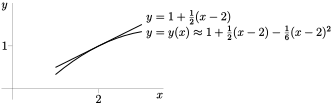
\includegraphics{graph18}
\end{center}
\end{answer}
\begin{solution}
$y$ is a function of $x$ that obeys
\begin{align*}
y(x)^4+xy(x)&=x^2-1
\intertext{
By implicit differentiation (and then subbing in $x=2$, $y(2)=1$)}
4y(x)^3y'(x)+y(x)+xy'(x)&=2x\\
 4y'(2)+1+2y'(2)&=4\\
  y'(2)&=\frac{1}{2}
\end{align*}
Differentiating with respect to $x$ a second time
and then subbing in\\ $x=2$, $y(2)=1$, $y'(2)=\frac{1}{2}$:
\begin{align*}
12y(x)^2y'(x)^2+4y(x)^3y''(x)+y'(x)+y'(x)+xy''(x)&=2\\
12\times1\times\frac{1}{4}+4y''(2)+\frac{1}{2}+\frac{1}{2}+2y''(2)&=2
\\ 6y''(2)&=-2\\
 y''(2)&=-\frac{1}{3}
\end{align*}The tangent line approximation to $y(x)$ at $x=2$ is
\begin{align*}
y(x)&\approx y(2)+y'(2)(x-2)=1+\frac{1}{2}(x-2)
\intertext{In particular,}
y(2.1)&\approx y(2)+y'(2)(2.1-2)=1+\frac{1}{2}(.1)=\boxed{1.05}
\intertext{The quadratic approximation to $y(x)$ at $x=2$ is}
y(x)&\approx y(2)+y'(2)(x-2)+\frac{1}{2} y''(2)(x-2)^2\\
&=1+\frac{1}{2}(x-2)-\frac{1}{6}(x-2)^2
\intertext{In particular, }
y(2.1)&\approx y(2)+y'(2)(2.1-2)+\frac{1}{2} y''(2)(2.1-2)^2\\
&=1+\frac{1}{2}(.1)-\frac{1}{6}(.1)^2=\boxed{1.0483}
\end{align*}
At $x=2$, $y=1$ and $y'=\frac{1}{2}$. So the tangent line passes through $(2,1)$
and has slope $\frac{1}{2}$. At $x=2$, $y''=-\frac{1}{3}$, so the graph $y=f(x)$
(locally!) looks like a parabola pointing down near $x=2$. This gives the graph fragment below.

Alternatively, we could observe that, near $x=2$, $y(x)$ will be quite close
to its quadratic approximation,
$1+\frac{1}{2}(x-2)-\frac{1}{6}(x-2)^2$.
\begin{center}
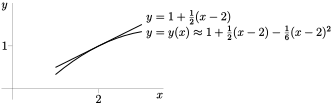
\includegraphics{graph18}
\end{center}
\end{solution}



\begin{question}[1996D]
The equation $x^4+y+xy^4=1$ defines $y$ implicitly as a function
of $x$ near the point $x=-1,~ y=1$.
\begin{enumerate}[(a)]
\item\label{s3.4tan1}  Use the tangent line approximation at the given point to
estimate the value of $y$ when $x=-0.9$.
\item\label{s3.4tan2}   Use the quadratic approximation  at the given point to get
another estimate of $y$ when $x=-0.9$.
\item\label{s3.4tan3} Make a sketch showing how
the curve relates to the tangent line at the given point.
\end{enumerate}
\end{question}
\begin{answer}
\eqref{s3.4tan1} 0.9\qquad
\eqref{s3.4tan2} {0.8867}\qquad
\eqref{s3.4tan3}
\begin{center}
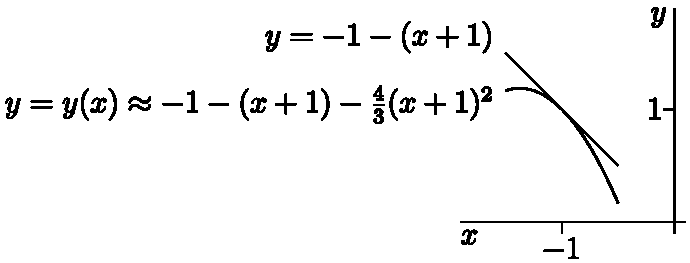
\includegraphics{graphE3b}
\end{center}\end{answer}
\begin{solution}
\eqref{s3.4tan1}
$y$ is a function of $x$ that obeys
\begin{align*}
1&=x^4+y(x)+xy(x)^4
\intertext{By implicit differentiation (and then subbing in $x=-1$, $y(-1)=1$)}
0&=4x^3+y'(x)+y(x)^4+4xy(x)^3y'(x)\\
0&= -4+y'(-1)+1-4y'(-1)\\
-1&= y'(-1)
\intertext{
Differentiating with respect to $x$ a second time
and then subbing in $x=-1$, $y(-1)=1$, and $y'(-1)=-1$:}
0&=12x^2+y''(x)+4y(x)^3y'(x)+4y(x)^3y'(x)+12xy(x)^2y'(x)^2+4xy(x)^3y''(x)\\
0&= 12+y''(-1)-4-4-12-4y''(-1)\\
-8&= 3y''(-1)\\
y''(-1)&=-\frac{8}{3}
\end{align*}
The tangent line approximation to $y(x)$ at $x=-1$ is
\begin{align*}
y(x)&\approx y(-1)+y'(-1)(x+1)=1-(x+1)=-x
\intertext{
In particular, }
y(-0.9)&\approx 0.9
\end{align*}
\eqref{s3.4tan2}
The quadratic approximation to $y(x)$ at $x=-1$ is
\begin{align*}
y(x)&\approx y(-1)+y'(-1)(x+1)+\frac{1}{2} y''(-1)(x+1)^2\\
&=1-(x+1)-\frac{4}{3}(x+1)^2
\intertext{In particular, }
y(-0.9)&\approx 1-(.1)-\frac{4}{3}(.1)^2\approx{0.8867}
\end{align*}
\eqref{s3.4tan3}
At $x=-1$, the slope of the curve is $y'(-1)=-1$. Its tangent line is falling
at $45^\circ$. At $x=-1$, $y''(-1)=-\frac{8}{3}$, so the slope of the
curve is decreasing as $x$ passes through $-1$. Zoomed in very close, the curve looks like a parabola opening downwards. This gives the figure
\begin{center}
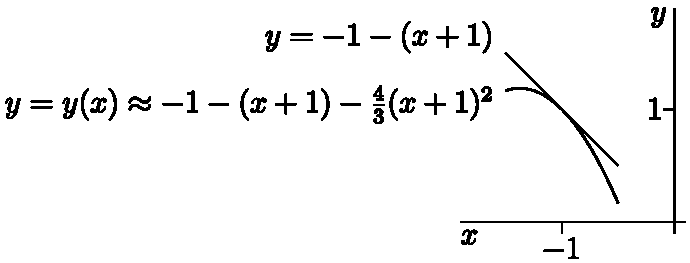
\includegraphics{graphE3b}
\end{center}\end{solution}

\begin{question}[1999H]
Given that $\log 10\approx 2.30259$, estimate $\log 10.3$ using
a suitable tangent line approximation. Give an upper and lower bound
for the error in your approximation by using a suitable error estimate.
\end{question}
\begin{answer}
$\log 10.3 \approx 2.33259$\\
The error is between
$-0.00045$ and $-0.00042$.
\end{answer}
\begin{solution}
 Let $f(x)=\log x$ and $x_0=10$. Then
\begin{align*}
f(x)&=\log x &
f'(x)&=\frac{1}{x} & f''(x)&=-\frac{1}{x^2} \\
f(10)&=\log 10\approx 2.30259 &
f'(10)&=\frac{1}{10} & f''(10)&=-\frac{1}{100}
\end{align*}
so that, with $x=10.3$,
$$
\log 10.3=f(10.3)\approx f(10)+f'(10)(10.3-10)
=2.30259+\frac{0.3}{10}
=2.33259
$$
The error in this approximation (excluding the error in the given data
$\log 10\approx 2.30259$) is $\dfrac{1}{2} f''(z)(10.3-10)^2$ for some $z$ between
$10$ and $10.3$. Because $f''(z)=-\dfrac{1}{z^2}$ increases as $z$ increases,
it must be between $-\dfrac{1}{10^2}$ and $-\dfrac{1}{10.3^2}$. This forces
$\dfrac{1}{2} f''(z)(10.3-10)^2$ to be between
$-\dfrac{1}{2}\cdot \dfrac{1}{10^2}(0.3)^2=-0.00045$ and
$-\dfrac{1}{2}\cdot \dfrac{1}{10.3^2}(0.3)^2<-0.00042$.
\end{solution}


\begin{question}[2012H]
Consider $f(x)=e^{e^x}$.
\begin{enumerate}[(a)]
\item Give the linear approximation for $f$ near $x=0$ (call this
$L(x)$).
\item Give the quadratic approximation for $f$ near $x=0$ (call
this $Q(x)$).
\item Prove that $L(x)<Q(x)<f(x)$ for all $x>0$.
\item Find an interval of length
at most $0.01$ that is guaranteed to contain the number $e^{0.1}$.
\end{enumerate}
\end{question}
\begin{hint} For (c), you can write $f(x)$ as the sum of $Q(x)$ and its error term.\\
For (d), you can use the linear approximation of $e^x$  centred at $0$, with its error term when $x=0.1$.
\end{hint}
\begin{answer}
(a) $L(x)=e+ex$ \qquad (b) $Q(x)=e+ex+ex^2$\\
(c) Since $ex^2 >0$ for all $x>0$, $L(x)<Q(x)$ for all $x>0$.

From the error formula, we know that
\begin{align*}
f(x)&=f(0)+f'(0)x+\half f''(0)x^2
+\dfrac{1}{3!}f'''(c)x^{3}\\
&=Q(x)+\frac{1}{6}\left(e^c+3e^{2c}+e^{3c}\right)e^{e^c}x^3
\end{align*}
for some $c$ between $0$ and $x$.
Since $\frac{1}{6}\left(e^c+3e^{2c}+e^{3c}\right)e^{e^c}$ is positive for any $c$, for
all $x>0$,
$\frac{1}{6}\left(e^c+3e^{2c}+e^{3c}\right)e^{e^c}x^3>0$, so
$Q(x)<f(x)$.

(d) $1.105<e^{0.1}<1.115$
\end{answer}
\begin{solution}
We begin by finding the values of the derivatives of $f$ at $x=0$. We can use the chain rule, or the formula we found in Question~\ref{s2.14expprod}, Section~\ref*{sec higher diff}.%2.14, higher order derivatives
\begin{align*}
f(x)&=e^{e^x}&f(0)&=e\\
f'(x)&=e^xe^{e^x}&f'(0)&=e\\
f''(x)&=\left(e^x+e^{2x}\right)e^{e^x}&f''(0)&=2e\\
f'''(x)&=\left(e^x+3e^{2x}+e^{3x}\right)e^{e^x}
\end{align*}

(a) $L(x)=f(0)+f'(0)(x-0)=e+ex$

(b) $Q(x)=f(0)+f'(0)(x-0)+\dfrac{1}{2}f''(0)(x-0)^2=e+ex+ex^2$

(c) Since $ex^2 >0$ for all $x>0$, $L(x)<Q(x)$ for all $x>0$.

From the error formula, we know that
\begin{align*}
f(x)&=f(0)+f'(0)x+\half f''(0)x^2
+\dfrac{1}{3!}f'''(c)x^{3}\\
&=Q(x)+\frac{1}{6}\left(e^c+3e^{2c}+e^{3c}\right)e^{e^c}x^3
\end{align*}
for some $c$ between $0$ and $x$.
Since $\frac{1}{6}\left(e^c+3e^{2c}+e^{3c}\right)e^{e^c}$ is positive for any $c$, for
all $x>0$,
$\frac{1}{6}\left(e^c+3e^{2c}+e^{3c}\right)e^{e^c}x^3>0$, so
$Q(x)<f(x)$.

(d) Write $g(x)=e^x=1+x+\dfrac{1}{2!}e^c x^2$, for some $c$ between
$0$ and $x$.
For $x=0.1$ we have $0<c<0.1$ and $1<e^c<e^{0.1}<e<3$.
So
\begin{align*}
e^{0.1}&&=&&f(0.1)&&=&&1+0.1+\half e^c (0.1)^2&&>&&1+0.1+\half (1) (0.1)^2&&=&&1.105\\
e^{0.1}&&=&&f(0.1)&&=&&1+0.1+\half e^c (0.1)^2&&<&&1+0.1+\half (3) (0.1)^2&&=&&1.115
\end{align*}
That is, $1.105<e^{0.1}<1.115$.
\end{solution}
